\documentclass[12pt, titlepage]{article}
\usepackage[utf8]{inputenc}
\usepackage[spanish]{babel}
\usepackage[letterpaper, margin=2.5cm]{geometry}
\usepackage{lipsum}
%\usepackage[nottoc,numbib]{tocbibind}
\usepackage{float}
\usepackage{amsmath}
\usepackage{url}
\usepackage{graphicx} 

\usepackage{listings}
\usepackage{color}
\definecolor{dkgreen}{rgb}{0,0.6,0}
\definecolor{gray}{rgb}{0.5,0.5,0.5}
\definecolor{mauve}{RGB}{253,151,31}

\lstset{frame=tb,
	aboveskip=3mm,
	belowskip=3mm,
	showstringspaces=false,
	columns=flexible,
	basicstyle={\small\ttfamily},
	numbers=none,
	numberstyle=\tiny\color{gray},
	keywordstyle=\color{blue},
	commentstyle=\color{dkgreen},
	stringstyle=\color{mauve},
	breaklines=true,
	breakatwhitespace=true,
	tabsize=3
}

\title{Reporte del segundo parcial}
\author{Carlos Tonatihu Barrera Pérez \\ Profesor: Genaro Juárez Martínez \\ Teoría Computacional \\ Grupo: 2CM4 }
\date{4 de diciembre de 2016}
\begin{document}
	\maketitle
	\tableofcontents
	
	\section{AFD Palabras que contienen 'web' y/o 'ebay'}
	\subsection{Descripción del problema}
	Cosas chidas
	\begin{figure}[H]
		\begin{center}
		\includegraphics[width=14cm, height=7cm]{img/webay.png}
		\caption{Diagrama de transiciones del autómata 'webay'.}
		\label{fig:diagrama1}
		\end{center}
	\end{figure}
	\subsection{Código}
	El código fue realizado en Python 3.5.
	\\Archivo: main\_webay.py
	\begin{lstlisting}[language=Python]
	print('main_webay.py')
	\end{lstlisting}
	\\Archivo: automata\_webay.py
	\begin{lstlisting}[language=Python]
	print('automata_webay.py')
	\end{lstlisting}
	\\Archivo: diagrama\_webay.py
	\begin{lstlisting}[language=Python]
	print('diagrama_webay.py')
	\end{lstlisting}
	\subsection{Pruebas}
	Pruebas de las opciones del menú.
	\\
	{\large Modo de consola.}
	\begin{figure}[H]
		\begin{center}
			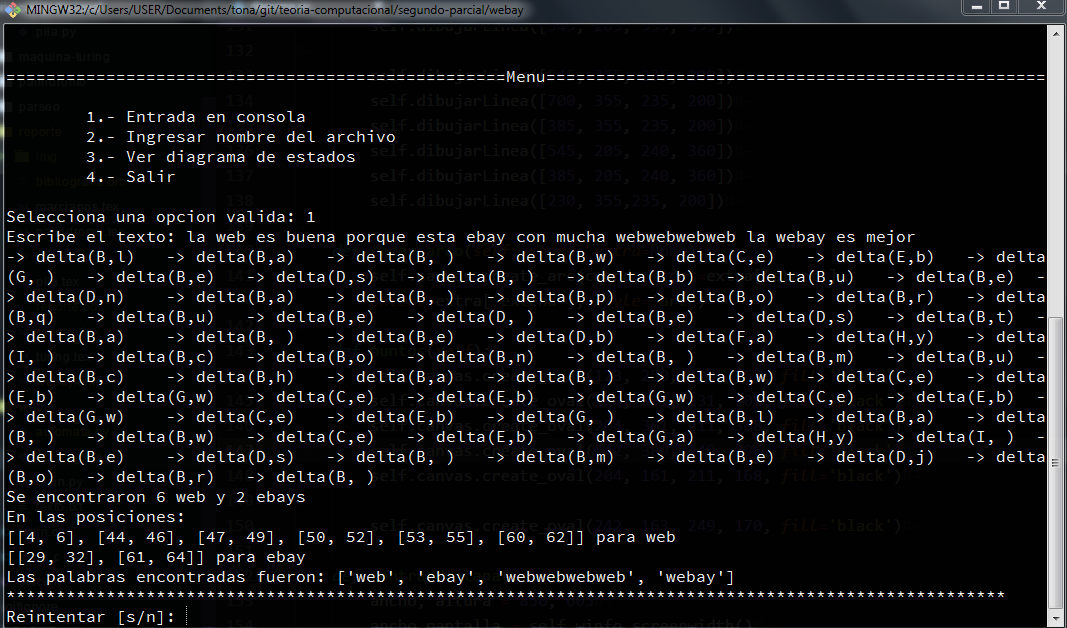
\includegraphics[width=\linewidth, height=6cm]{img/webay-manual.png}
			\caption{Historia del autómata y las palabras con 'web' y/o 'ebay'.}
			\label{fig:webay1}
		\end{center}
	\end{figure}
	{\large Modo archivo.}
	\begin{figure}[H]
		\begin{center}
			\includegraphics[width=\linewidth, height=20cm]{img/webay-automatico.png}
			\caption{Parte de la historia del autómata y las palabras con 'web' y/o 'ebay'.}
			\label{fig:webay2}
		\end{center}
	\end{figure}
	{\large Diagrama.}
	\begin{figure}[H]
		\begin{center}
			\includegraphics[width=\linewidth, height=9cm]{img/diagrama-webay.png}
			\caption{Diagrama de transiciones del autómata 'webay'.}
			\label{fig:webay3}
		\end{center}
	\end{figure}
	%\section{Planetas}
	\subsection{Descripción del problema}
	Se desarrollo un programa para observar en que momento falla el tener $n$ numero de elementos en 3 grupos, se le llama fallar al punto en el que solo hay elementos en uno de los grupos.
	El procedimiento se realiza tomando 1 elemento de dos de los grupos y así obtener 2 nuevos elementos en el otro conjunto como en la figura \ref{fig:marcianos}.
	\begin{figure}[H]
		\begin{center}
			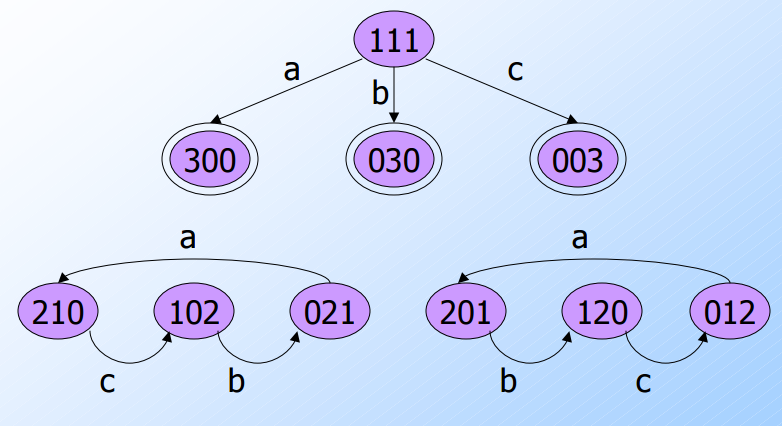
\includegraphics[width=10cm, height=4cm]{img/marcianos.png}
			\caption{Ejemplo de funcionamiento con 3 elementos.\cite{WEB}}
			\label{fig:marcianos}
		\end{center}
	\end{figure}
	Se mostraran los diferentes caminos que puede tomar el proceso al introducir el numero de los elementos. El programa cuenta con modo manual y automático.
	\subsection{Código}
	El código fue realizado en C.
	\\Archivo: arbol.h
	\begin{lstlisting}[language=C]
	#ifndef __ARBOL__
	#define __ARBOL__

	#include <stdio.h>
	#include <stdlib.h>

	struct Nodos{
	  int dato[3];
	  struct Nodos *siguiente;
	};

	typedef struct Nodos Nodo;

	struct Arbol{
	  int elemento[3];
	  struct Arbol *arbolA;
	  struct Arbol *arbolB;
	  struct Arbol *arbolC;
	  Nodo *primero;
	};
	int insertar(struct Arbol **, int[3], Nodo *, int);
	int crear_arbol(struct Arbol **, int[3], Nodo *);
	void imprimir_arbol(struct Arbol *, int);

	#endif
	\end{lstlisting}
	Archivo: arbol.c
	\begin{lstlisting}[language=C]
		#include "arbol.h"
		int insertar(struct Arbol **arbol, int valor[3], Nodo *lista, int continuar) {
		    int valor_aux[3];
		    struct Arbol *arbol_nuevo = NULL;
		    if(arbol == NULL) {
		        return -1; //No existe
		    }
		    int existe_arbol_nuevo = crear_arbol(&arbol_nuevo, valor, lista);
		    if(existe_arbol_nuevo==-1) {
		        return -1; // No existe
		    }
		    if (*arbol == NULL) {
		        *arbol = arbol_nuevo; //Raiz
		    }
		    if (continuar == 0){
		        return 1;
		    }
		    if (valor[1] > 0 && valor[2] > 0) {
		        int repetido =0;
		        valor_aux[1] = valor[1] - 1;
		        valor_aux[2] = valor[2] - 1;
		        valor_aux[0] = valor[0] + 2;
		        Nodo *mas = arbol_nuevo->primero;
		        while(mas != NULL){
		            if((mas->dato[0] == valor_aux[0])&&(mas->dato[1] == valor_aux[1])&&(mas->dato[2] == valor_aux[2])) {
		                repetido = 1;
		                break;
		            }
		            mas = mas->siguiente;
		        }
		        if (repetido == 0){
		            insertar(&((*arbol)->arbolA), valor_aux, arbol_nuevo->primero, 1);
		        } else{
		            insertar(&((*arbol)->arbolA), valor_aux, arbol_nuevo->primero, 0);
		        }
		    }
		    if (valor[0] > 0 && valor[2] > 0) {
		        int repetido =0;
		        valor_aux[0] = valor[0] - 1;
		        valor_aux[2] = valor[2] - 1;
		        valor_aux[1] = valor[1] + 2;
		        Nodo *mas = arbol_nuevo->primero;
		        while(mas != NULL){
		            if((mas->dato[0] == valor_aux[0])&&(mas->dato[1] == valor_aux[1])&&(mas->dato[2] == valor_aux[2])) {
		                repetido = 1;
		                break;
		            }
		            mas = mas->siguiente;
		        }
		        if (repetido == 0){
		            insertar(&((*arbol)->arbolB), valor_aux, arbol_nuevo->primero, 1);
		        } else{
		            insertar(&((*arbol)->arbolB), valor_aux, arbol_nuevo->primero, 0);
		        }
		    }
		    if (valor[0] > 0 && valor[1] > 0) {
		        int repetido =0;
		        valor_aux[0] = valor[0] - 1;
		        valor_aux[1] = valor[1] - 1;
		        valor_aux[2] = valor[2] + 2;
		        Nodo *mas = arbol_nuevo->primero;
		        while(mas != NULL){
		            if((mas->dato[0] == valor_aux[0])&&(mas->dato[1] == valor_aux[1])&&(mas->dato[2] == valor_aux[2])) {
		                repetido = 1;
		                break;
		            } else{
		            }
		            mas = mas->siguiente;
		        }
		        if (repetido == 0){
		            insertar(&((*arbol)->arbolC), valor_aux, arbol_nuevo->primero, 1);
		        } else{
		            insertar(&((*arbol)->arbolC), valor_aux, arbol_nuevo->primero, 0);
		        }

		    }
		    return 1;
		}

		int crear_arbol(struct Arbol **nuevo, int valor[3], Nodo *lista) {
		    struct Arbol *auxiliar = NULL;
		    auxiliar = (struct Arbol*)malloc(sizeof(struct Arbol));
		    if (auxiliar == NULL) {
		        return -1;
		    }
		    auxiliar->arbolA = NULL;
		    auxiliar->arbolB = NULL;
		    auxiliar->arbolC = NULL;
		    auxiliar->elemento[0] = valor[0];
		    auxiliar->elemento[1] = valor[1];
		    auxiliar->elemento[2] = valor[2];
		    auxiliar->primero = NULL;

		    while(lista != NULL){
		        Nodo **final_lista = &(auxiliar->primero);
		        while(*final_lista != NULL){
		            final_lista = &((*final_lista)->siguiente);
		        }

		        Nodo *temporal = NULL;
		        temporal = (Nodo *) malloc(sizeof(Nodo));
		        if (temporal == NULL){
		            printf("Temporal es null");
		        }
		        temporal->dato[0] = lista->dato[0];
		        temporal->dato[1] = lista->dato[1];
		        temporal->dato[2] = lista->dato[2];
		        temporal->siguiente = NULL;

		        *final_lista = temporal;
		        lista = lista->siguiente;
		    }

		    Nodo **final = &(auxiliar->primero);
		    while(*final != NULL){
		        final = &((*final)->siguiente);
		    }

		    Nodo *temporal = NULL;
		    temporal = (Nodo *) malloc(sizeof(Nodo));
		    if (temporal == NULL){
		        printf("Temporal es null");
		    }
		    temporal->dato[0] = valor[0];
		    temporal->dato[1] = valor[1];
		    temporal->dato[2] = valor[2];
		    temporal->siguiente = NULL;

		    *final = temporal;
		    *nuevo = auxiliar;
		    return 1;
		}
		void imprimir_arbol(struct Arbol *arbol, int n){
		    int contador = 0;
		    if(arbol->arbolA != NULL){
		        imprimir_arbol(arbol->arbolA, n);
		    } else {
		        contador = contador +1;
		    }

		    if(arbol->arbolB != NULL){
		        imprimir_arbol(arbol->arbolB, n);
		    } else {
		        contador = contador +1;
		    }
		    if(arbol->arbolC != NULL){
		        imprimir_arbol(arbol->arbolC, n);
		    } else {
		        contador = contador +1;
		    }
		    if (contador == 3){
		        FILE *archivo = NULL;
		        archivo = fopen("resultado.txt", "a");
		        Nodo *mi_nodo = arbol->primero;
		        while(mi_nodo !=NULL){
		            fprintf(archivo, "[%d,", mi_nodo->dato[0]);
		            fprintf(archivo, "%d,", mi_nodo->dato[1]);
		            fprintf(archivo, "%d]", mi_nodo->dato[2]);
		            fputc(' ', archivo);
		            if(mi_nodo->siguiente ==NULL){
		                if(mi_nodo->dato[0] == n || mi_nodo->dato[1] == n || mi_nodo->dato[2] == n){
		                    fputs("--Falla-- ", archivo);
		                }
		            }
		            mi_nodo = mi_nodo->siguiente;
		        }
		        fputs("\n", archivo);
		        fclose(archivo);
		    }

		}
	\end{lstlisting}
	Archivo: main\_planetas.c
	\begin{lstlisting}[language=C]
		#include <stdio.h>
		#include <stdlib.h>
		#include <time.h>
		#include "arbol.h"
		int menu() {
		    int opcion;
		    printf("Que quieres hacer?\n1.-Manual\n2.-Automatico\n3.-Salir\n");
		    scanf(" %d", &opcion);
		    return opcion;
		}

		int menu_continuar() {
		    int opcion;
		    printf("Intentar otra vez?\nSi = 1 NO = 0\n");
		    scanf(" %d", &opcion);
		    return opcion;
		}

		int random_longitud() {
		    int longitud = 1 + rand() % (1000 + 1 - 1);
		    return longitud;
		}

		void iniciar(int n){
		    FILE *archivo = NULL;
		    archivo = fopen("resultado.txt", "w");
		    fprintf(archivo, "El numero de elementos es:%d \n", n);
		    fclose(archivo);
		    srand(time(NULL));

		    int a = 0;
		    int b = 0;
		    int c = 0;

		    while(1){
		        a = n-b;
		        while(1){
		            int numero[3];
		            struct Arbol *arbol_prueba = NULL;
		            Nodo *lista = NULL;
		            archivo = fopen("resultado.txt", "a");
		            numero[0] = a;
		            numero[1] = b;
		            numero[2] = c;
		            insertar(&arbol_prueba, numero, lista, 1);
		            fputs("Combinacion: ", archivo);
		            fprintf(archivo, "[%d,", numero[0]);
		            fprintf(archivo, "%d,", numero[1]);
		            fprintf(archivo, "%d]\n", numero[2]);
		            fclose(archivo);
		            imprimir_arbol(arbol_prueba, n);
		            a = a-1;
		            c = c+1;
		            if (a<0){
		                break;
		            }
		        }
		        b = b+1;
		        c = 0;
		        if (b == n+1){
		            break;
		        }
		    }
		}

		int main(int argc, char const *argv[]) {
		    int continuar = 1;
		    int manual = 1;
		    int longitud = 0;
		    while(continuar) {
		        manual = menu();
		        if (manual == 1) {
		            printf("%s\n", "Ingresa el numero de elementos  en el intervalo [0-1000]: ");
		            scanf("%d", &longitud);
		        } else if (manual == 2) {
		            longitud = random_longitud();
		        } else {
		            break;
		        }
		        printf("El numero de elementos es: %d\n", longitud);
		        iniciar(longitud);
		        printf("Proceso terminado, revisar archivo resultado.txt\n");
		        continuar = menu_continuar();
		    }
		    return 0;
		}

	\end{lstlisting}
	\subsection{Pruebas}
	Pruebas de las opciones del menú.
	\\
	{\large Modo de manual.}
	\begin{figure}[H]
		\begin{center}
			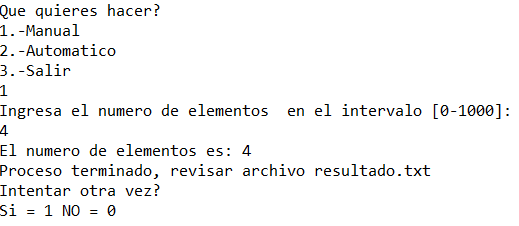
\includegraphics[width=10cm, height=5cm]{img/marcianos-manual-consola.png}
			\caption{Ejecución del programa en modo manual.}
			\label{fig:marcianos1}
		\end{center}
	\end{figure}
	\begin{figure}[H]
		\begin{center}
			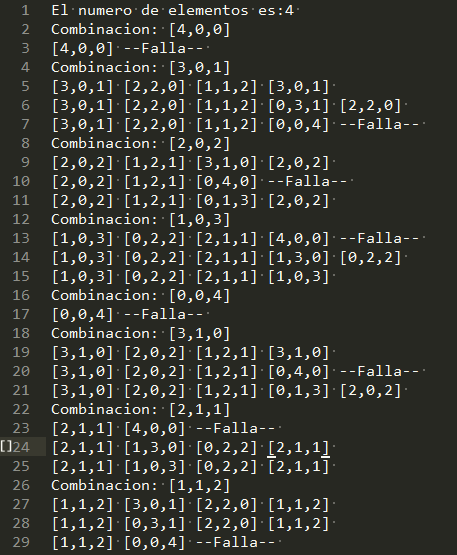
\includegraphics[width=9cm, height=10cm]{img/marcianos-manual-archivo1.png}
			\caption{Resultado del proceso parte 1.}
			\label{fig:marcianos2a}
		\end{center}
	\end{figure}
\begin{figure}[H]
	\begin{center}
		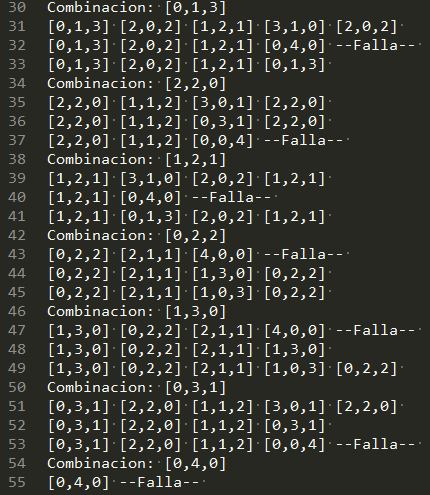
\includegraphics[width=9cm, height=10cm]{img/marcianos-manual-archivo2.png}
		\caption{Resultado del proceso parte 2.}
		\label{fig:marcianos2b}
	\end{center}
\end{figure}
	{\large Modo automático}
	\begin{figure}[H]
		\begin{center}
			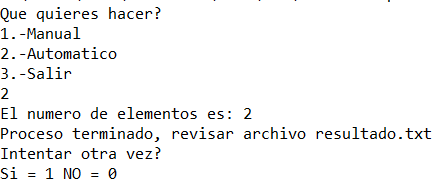
\includegraphics[width=\linewidth, height=7cm]{img/marcianos-automatico-consola.png}
			\caption{Probando el modo automático}
			\label{fig:marcianos3}
		\end{center}
	\end{figure}
	\begin{figure}[H]
		\begin{center}
			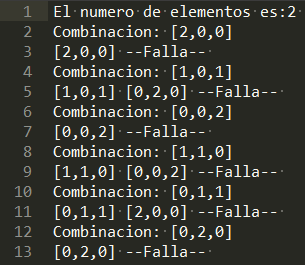
\includegraphics[width=8cm, height=7cm]{img/marcianos-automatico-archivo.png}
			\caption{Resultado de la prueba}
			\label{fig:marcianos4}
		\end{center}
	\end{figure}

	\section{Palindromo usando gramáticas}
	\subsection{Descripción del problema}
	Cosas chidas
	\begin{figure}[H]
		\begin{center}
		\includegraphics[width=14cm, height=7cm]{img/palindromo.png}
		\caption{Ejemplo de un palindromo binario}
		\label{fig:diagrama-palindromo}
		\end{center}
	\end{figure}
	\subsection{Código}
	El código fue realizado en Python 3.5.
	\\Archivo: main\_palindromo.py
	\begin{lstlisting}[language=Python]
	print('main_palindromo.py')
	\end{lstlisting}
	\\Archivo: palindromo.py
	\begin{lstlisting}[language=Python]
	print('palindromo.py')
	\end{lstlisting}
	\subsection{Pruebas}
	Pruebas de las opciones del menú.
	\\
	{\large Modo de automatico.}
	\begin{figure}[H]
		\begin{center}
			\includegraphics[width=\linewidth, height=6cm]{img/palindromo.png}
			\caption{Historia de la generación del palindromo.}
			\label{fig:palindromo1}
		\end{center}
	\end{figure}
	\section{AFD Palabras que contienen 'web' y/o 'ebay'}
	\subsection{Descripción del problema}
	Cosas chidas
	\begin{figure}[H]
		\begin{center}
		\includegraphics[width=14cm, height=7cm]{img/webay.png}
		\caption{Diagrama de transiciones del autómata 'webay'.}
		\label{fig:diagrama1}
		\end{center}
	\end{figure}
	\subsection{Código}
	El código fue realizado en Python 3.5.
	\\Archivo: main\_webay.py
	\begin{lstlisting}[language=Python]
	print('main_webay.py')
	\end{lstlisting}
	\\Archivo: automata\_webay.py
	\begin{lstlisting}[language=Python]
	print('automata_webay.py')
	\end{lstlisting}
	\\Archivo: diagrama\_webay.py
	\begin{lstlisting}[language=Python]
	print('diagrama_webay.py')
	\end{lstlisting}
	\subsection{Pruebas}
	Pruebas de las opciones del menú.
	\\
	{\large Modo de consola.}
	\begin{figure}[H]
		\begin{center}
			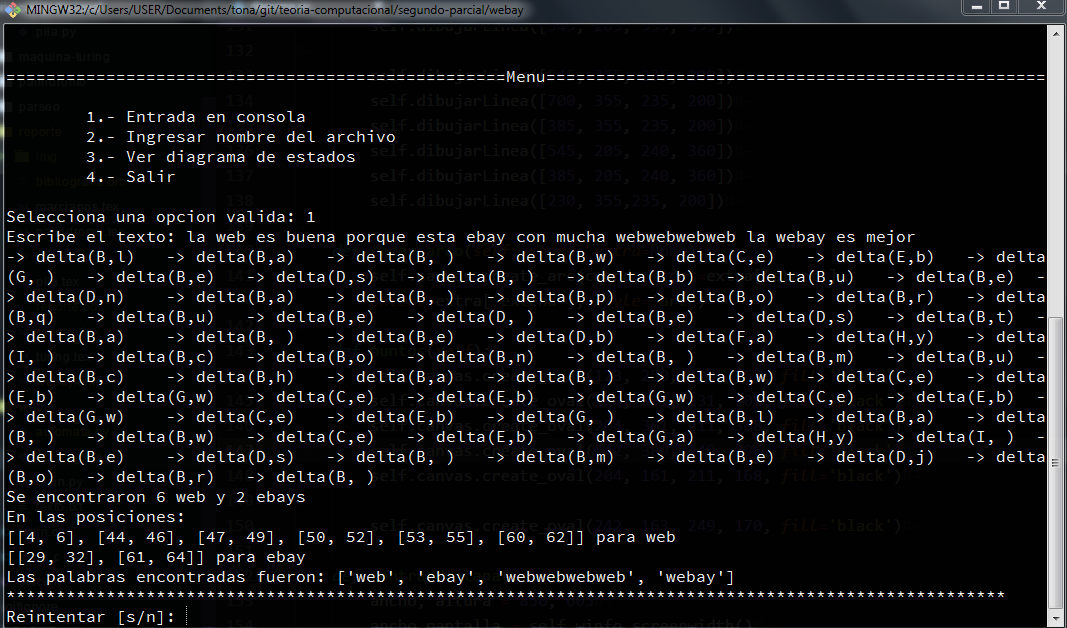
\includegraphics[width=\linewidth, height=6cm]{img/webay-manual.png}
			\caption{Historia del autómata y las palabras con 'web' y/o 'ebay'.}
			\label{fig:webay1}
		\end{center}
	\end{figure}
	{\large Modo archivo.}
	\begin{figure}[H]
		\begin{center}
			\includegraphics[width=\linewidth, height=20cm]{img/webay-automatico.png}
			\caption{Parte de la historia del autómata y las palabras con 'web' y/o 'ebay'.}
			\label{fig:webay2}
		\end{center}
	\end{figure}
	{\large Diagrama.}
	\begin{figure}[H]
		\begin{center}
			\includegraphics[width=\linewidth, height=9cm]{img/diagrama-webay.png}
			\caption{Diagrama de transiciones del autómata 'webay'.}
			\label{fig:webay3}
		\end{center}
	\end{figure}
	\section{Autómata de Pila}
	\subsection{Descripción del problema}
	En este programa se desarrollo un autómata de pila (vease figura \ref{fig:diagrama-pila}) que aceptara el lenguaje de $ \left\lbrace 0^{n}1^{n} \mid n\geq 1\right\rbrace  $. El programa tiene un modo manual y automático en ambos modos se evalúa una cadena de ceros y unos de longitud $1 \le n \le 1000 $ y se muestra si la cadena es valida o no junto con los pasos para llegar a este resultado que se mostraran en archivo y consola.
	Además, se puede observar la animación de este proceso como el de la figura \ref{pila-animacion} si así se desea, esta acción remplaza a la historia del autómata en consola pero no en archivo.
	\begin{figure}[H]
		\begin{center}
		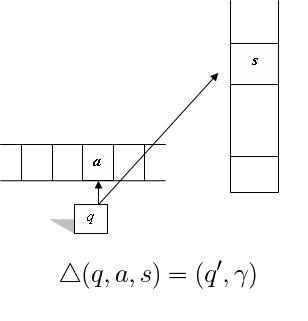
\includegraphics[width=9cm, height=6cm]{img/automata-pila.png}
		\caption{Representación de un autómata de Pila.}
		\label{fig:diagrama-pila}
		\end{center}
	\end{figure}
	\begin{figure}[H]
		\begin{center}
			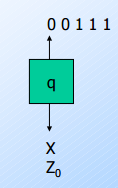
\includegraphics[width=6cm, height=6cm]{img/animacion-pila.png}
			\caption{Representación de un autómata de Pila.}
			\label{fig:pila-animacion}
		\end{center}
	\end{figure}
	\subsection{Código}
	El código fue realizado en Python 3.5.
	\\Archivo: main\_pila.py
	\begin{lstlisting}[language=Python]
	#main_pila.py
	# -*- coding: utf-8 -*-
	from __future__ import print_function
	from pila import automata
	import random

	separador = '='*50
	def iniciar():
	    continuar = True
	    while continuar:
	        opcion = imprimir_menu()
	        if opcion == 1:
	            entrada_consola()
	        elif opcion == 2:
	            ejecutar_random()
	        else:
	            break # Sal del programa
	        print('=' * 100)
	        opcion = input("Reintentar [s/n]: ")
	        if opcion.lower() != 's':
	            continuar = False

	    print('Saliendo del programa...')

	def imprimir_menu():
	    print('\n\n%sMenu%s' % (separador, separador))
	    print("""
	        1.- Entrada en consola (Manual)
	        2.- Aleatorio (Automatico)
	        3.- Salir
	    """)
	    try:
	        opcion = int(input("Selecciona una opcion valida: "))
	        return opcion
	    except Exception as e:
	        print('Error ', e)
	        return 0

	def entrada_consola():
	    texto = input("Escribe el numero binario: ")
	    animacion = ver_animacion()
	    automata(texto, animacion)

	def ver_animacion():
	    opcion = input("Ver animacion [s/n]: ")
	    if opcion == 's':
	        return True
	    else:
	        return False

	def ejecutar_random():
	    i = 0
	    longitud_random = random.randint(1, 10)
	    numero_binario = ''
	    while i < longitud_random:
	        numero_binario += random.choice(['0', '1'])
	        i += 1

	    print("El numero aleatorio es: ", numero_binario)
	    animacion = ver_animacion()
	    automata(numero_binario, animacion)

	iniciar()
	\end{lstlisting}
	Archivo: automata\_pila.py
	\begin{lstlisting}[language=Python]
	#automata_pila.py
	# -*- coding: utf-8 -*-
	from __future__ import print_function
	import time

	class Pila(object):
	    def __init__(self):
	        self.altura = -1
	        self.elementos = []

	    def vacio(self):
	        if self.altura == -1:
	            return True
	        else:
	            return False

	    def sacar(self):
	        if self.vacio():
	            return 'e'
	        else:
	            valor = self.elementos[self.altura]
	            self.altura -= 1
	            return valor

	    def meter(self, elemento):
	        self.altura += 1
	        self.elementos[self.altura:] = [elemento]

	    def mostrar(self):
	        i = self.altura
	        cadena = ''
	        while(i>-1):
	            cadena += self.elementos[i]
	            i -= 1
	        return cadena

	def automata(cadena, ver_animacion):
	    pila = Pila()
	    archivo = open('historia-pila.txt', 'w')
	    pila.meter('Zo')
	    estado = 'q'
	    cadena_aux = cadena
	    cadena = cadena + ' '
	    archivo.write('La cadena es: ' + cadena_aux + '\n')
	    for simbolo in cadena:
	        if cadena_aux == '':
	            cadena_aux = 'e'
	        if ver_animacion:
	            time.sleep(1)
	            pintar(estado, cadena_aux, pila)
	        else:
	            print('(%s, %s, %s)' %(estado, cadena_aux, pila.mostrar()), end=' |- ')
	        archivo.write('(%s, %s, %s) |- ' %(estado, cadena_aux, pila.mostrar()))
	        if estado == 'q':
	            if simbolo == '0':
	                pila.meter('X')
	            elif simbolo == '1':
	                if pila.sacar() == 'Zo':
	                    pila.meter('Zo')
	                    break
	                estado = 'p'
	            else:
	                estado = 'f'
	                break
	        elif estado == 'p':
	            if simbolo == '1':
	                if pila.sacar() == 'Zo':
	                    estado = 'f'
	                    pila.meter('Zo')
	                    break
	            elif simbolo == '0':
	                pila.meter('X')
	                cadena_aux = cadena_aux[1:]
	                break
	            elif simbolo == ' ':
	                estado = 'f'
	                if pila.mostrar() == 'Zo':
	                    break
	        cadena_aux = cadena_aux[1:]

	    if cadena_aux == '':
	        cadena_aux = 'e'
	    if ver_animacion:
	        time.sleep(1)
	        pintar(estado, cadena_aux, pila)
	    else:
	        print('(%s, %s, %s)' %(estado, cadena_aux, pila.mostrar()))
	        print('\n')
	    archivo.write('(%s, %s, %s)' %(estado, cadena_aux, pila.mostrar()))
	    if (pila.mostrar() == 'Zo') and cadena_aux == 'e':
	        print('\nCadena valida')
	        archivo.write('\nCadena valida')
	    else:
	        print('\nCadena invalida')
	        archivo.write('\nCadena invalida')
	    archivo.close()

	def pintar(estado, cadena_aux, stack):
	    pila = 'Zo'
	    if stack.mostrar() != '':
	        pila = stack.mostrar()

	    print('\n')
	    print('\n')
	    print('\n')
	    print('\n')
	    print('\n')
	    print('     %s' %cadena_aux)
	    print('     ^')
	    print('     |')
	    print('     |')
	    print('     |')
	    print('-----------')
	    print('|         |')
	    print('|    %s    |' %estado)
	    print('|         |')
	    print('-----------')
	    print('     |')
	    print('     |')
	    print('     |')
	    print('     v')
	    print('     %s' %pila)
	    print('\n')
	    print('\n')
	    print('\n')
	    print('\n')
	    print('\n')
	\end{lstlisting}
	\subsection{Pruebas}
	Pruebas de las opciones del menú.
	\\
	{\large Modo de manual.}
	\begin{figure}[H]
		\begin{center}
			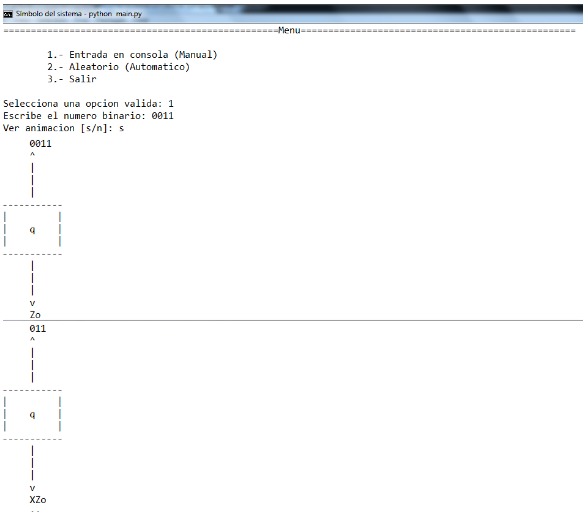
\includegraphics[width=14cm, height=12cm]{img/pila-manual-consola1.png}
			\caption{Historia del Autómata de Pila en animación 1}
			\label{fig:pila1a}
		\end{center}
	\end{figure}
	\begin{figure}[H]
		\begin{center}
			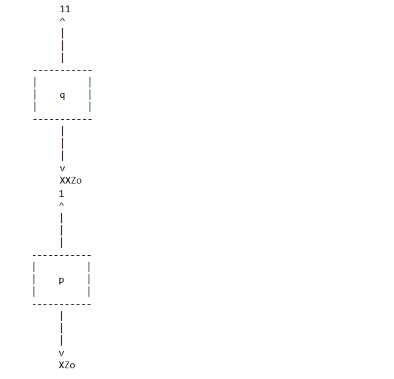
\includegraphics[width=14cm, height=10cm]{img/pila-manual-consola2.png}
			\caption{Historia del Autómata de Pila en animación 2}
			\label{fig:pila1b}
		\end{center}
	\end{figure}
	\begin{figure}[H]
		\begin{center}
			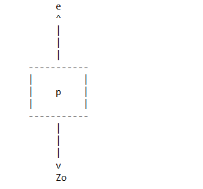
\includegraphics[width=7cm, height=7cm]{img/pila-manual-consola3.png}
			\caption{Historia del Autómata de Pila en animación 3}
			\label{fig:pila1c}
		\end{center}
	\end{figure}
	\begin{figure}[H]
		\begin{center}
			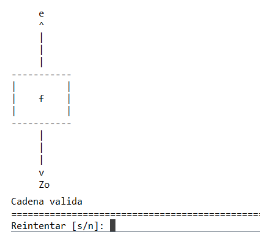
\includegraphics[width=9cm, height=8cm]{img/pila-manual-consola4.png}
			\caption{Historia del Autómata de Pila en animación 4}
			\label{fig:pila1d}
		\end{center}
	\end{figure}
	\begin{figure}[H]
		\begin{center}
			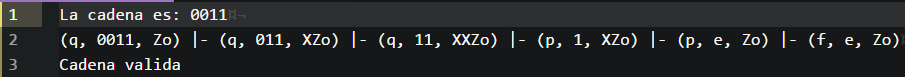
\includegraphics[width=\linewidth, height=3cm]{img/pila-manual-archivo.png}
			\caption{Historia del Autómata de Pila.}
			\label{fig:pila2}
		\end{center}
	\end{figure}
	\newpage
	{\large Modo automático}
	\begin{figure}[H]
		\begin{center}
			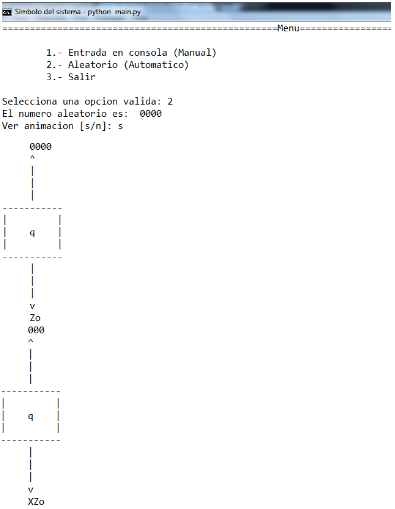
\includegraphics[width=14cm, height=16cm]{img/pila-automatico-consola1.png}
			\caption{Historia del Autómata de Pila en animación 1}
			\label{fig:pila2a}
		\end{center}
	\end{figure}
	\begin{figure}[H]
		\begin{center}
			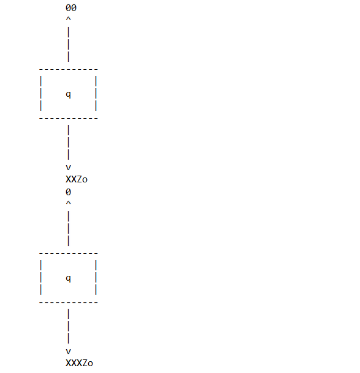
\includegraphics[width=14cm, height=12cm]{img/pila-automatico-consola2.png}
			\caption{Historia del Autómata de Pila en animación 2}
			\label{fig:pila2b}
		\end{center}
	\end{figure}
	\begin{figure}[H]
		\begin{center}
			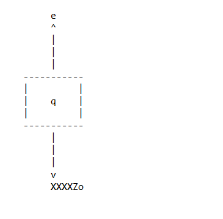
\includegraphics[width=7cm, height=7cm]{img/pila-automatico-consola3.png}
			\caption{Historia del Autómata de Pila en animación 3}
			\label{fig:pila2c}
		\end{center}
	\end{figure}
	\begin{figure}[H]
		\begin{center}
			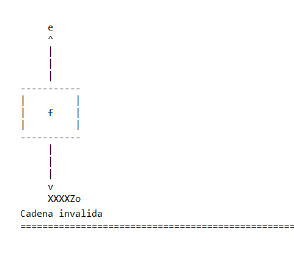
\includegraphics[width=9cm, height=8cm]{img/pila-automatico-consola4.png}
			\caption{Historia del Autómata de Pila en animación 4}
			\label{fig:pila2d}
		\end{center}
	\end{figure}
	\begin{figure}[H]
		\begin{center}
			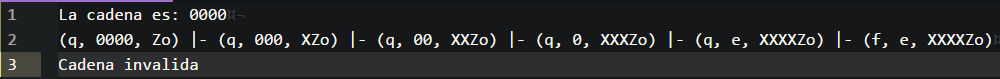
\includegraphics[width=\linewidth, height=3cm]{img/pila-automatico-archivo.png}
			\caption{Historia del Autómata de Pila en archivo.}
			\label{fig:pila4}
		\end{center}
	
	\end{figure}

	\section{Maquina de Turing}
	\subsection{Descripción del problema}
	Cosas chidas
	\begin{figure}[H]
		\begin{center}
		\includegraphics[width=14cm, height=7cm]{img/turing.png}
		\caption{Representación de una Maquina de Turing}
		\label{fig:diagrama-turing}
		\end{center}
	\end{figure}
	\subsection{Código}
	El código fue realizado en Python 3.5.
	\\Archivo: main\_turing.py
	\begin{lstlisting}[language=Python]
	print('main_turing.py')
	\end{lstlisting}
	\\Archivo: maquina\_turing.py
	\begin{lstlisting}[language=Python]
	print('maquina de turing.py')
	\end{lstlisting}
	\subsection{Pruebas}
	Pruebas de las opciones del menú.
	\\
	{\large Modo de consola.}
	\begin{figure}[H]
		\begin{center}
			\includegraphics[width=\linewidth, height=6cm]{img/turing-manual.png}
			\caption{Historia de la Maquina de Turing.}
			\label{fig:turing1}
		\end{center}
	\end{figure}
	{\large Modo archivo.}
	\begin{figure}[H]
		\begin{center}
			\includegraphics[width=\linewidth, height=20cm]{img/turing-automatico.png}
			\caption{Parte de la historia de la Maquina de Turing.}
			\label{fig:turing2}
		\end{center}
	\end{figure}
	\bibliography{bibliografia} 
	\bibliographystyle{ieeetr}
\end{document}